%%%%%%%%%%%%%%%%%%%%%%%%%%%%%%%%%%%%%%%%%%%%%%%%%%%%%%%%%%%%%%%%%%%%%%%%%%%
% Relational algebra & relational calculus for Sailer-Reserve-Boat
% schema in the DBMS book.
% Author: Shuo Yang
%%%%%%%%%%%%%%%%%%%%%%%%%%%%%%%%%%%%%%%%%%%%%%%%%%%%%%%%%%%%%%%%%%%%%%%%%%%

\documentclass[10pt]{article}
\usepackage{amsmath,amssymb,epsfig,graphics,hyperref,amsthm,mathtools}
\DeclarePairedDelimiter\ceil{\lceil}{\rceil}
\DeclarePairedDelimiter\floor{\lfloor}{\rfloor}

\hypersetup{colorlinks=true}

\setlength{\textwidth}{7in}
\setlength{\topmargin}{-0.575in}
\setlength{\textheight}{9.25in}
\setlength{\oddsidemargin}{-.25in}
\setlength{\evensidemargin}{-.25in}

\reversemarginpar
\setlength{\marginparsep}{-15mm}

\newcommand{\rmv}[1]{}
\newcommand{\bemph}[1]{{\bfseries\itshape#1}}
\newcommand{\N}{\mathbb{N}}
\newcommand{\Z}{\mathbb{Z}}
\newcommand{\imply}{\to}
\newcommand{\bic}{\leftrightarrow}

\def\Author{Shuo Yang}

\begin{document}

\noindent

\begin{center}
  CS460-Prog4: Sample Design\\
  \Author\\
\end{center}

% A horizontal split line
\hrule\smallskip

\vspace{1em}
\underline{Conceptual Design/ER Diagram}:
\begin{center}
  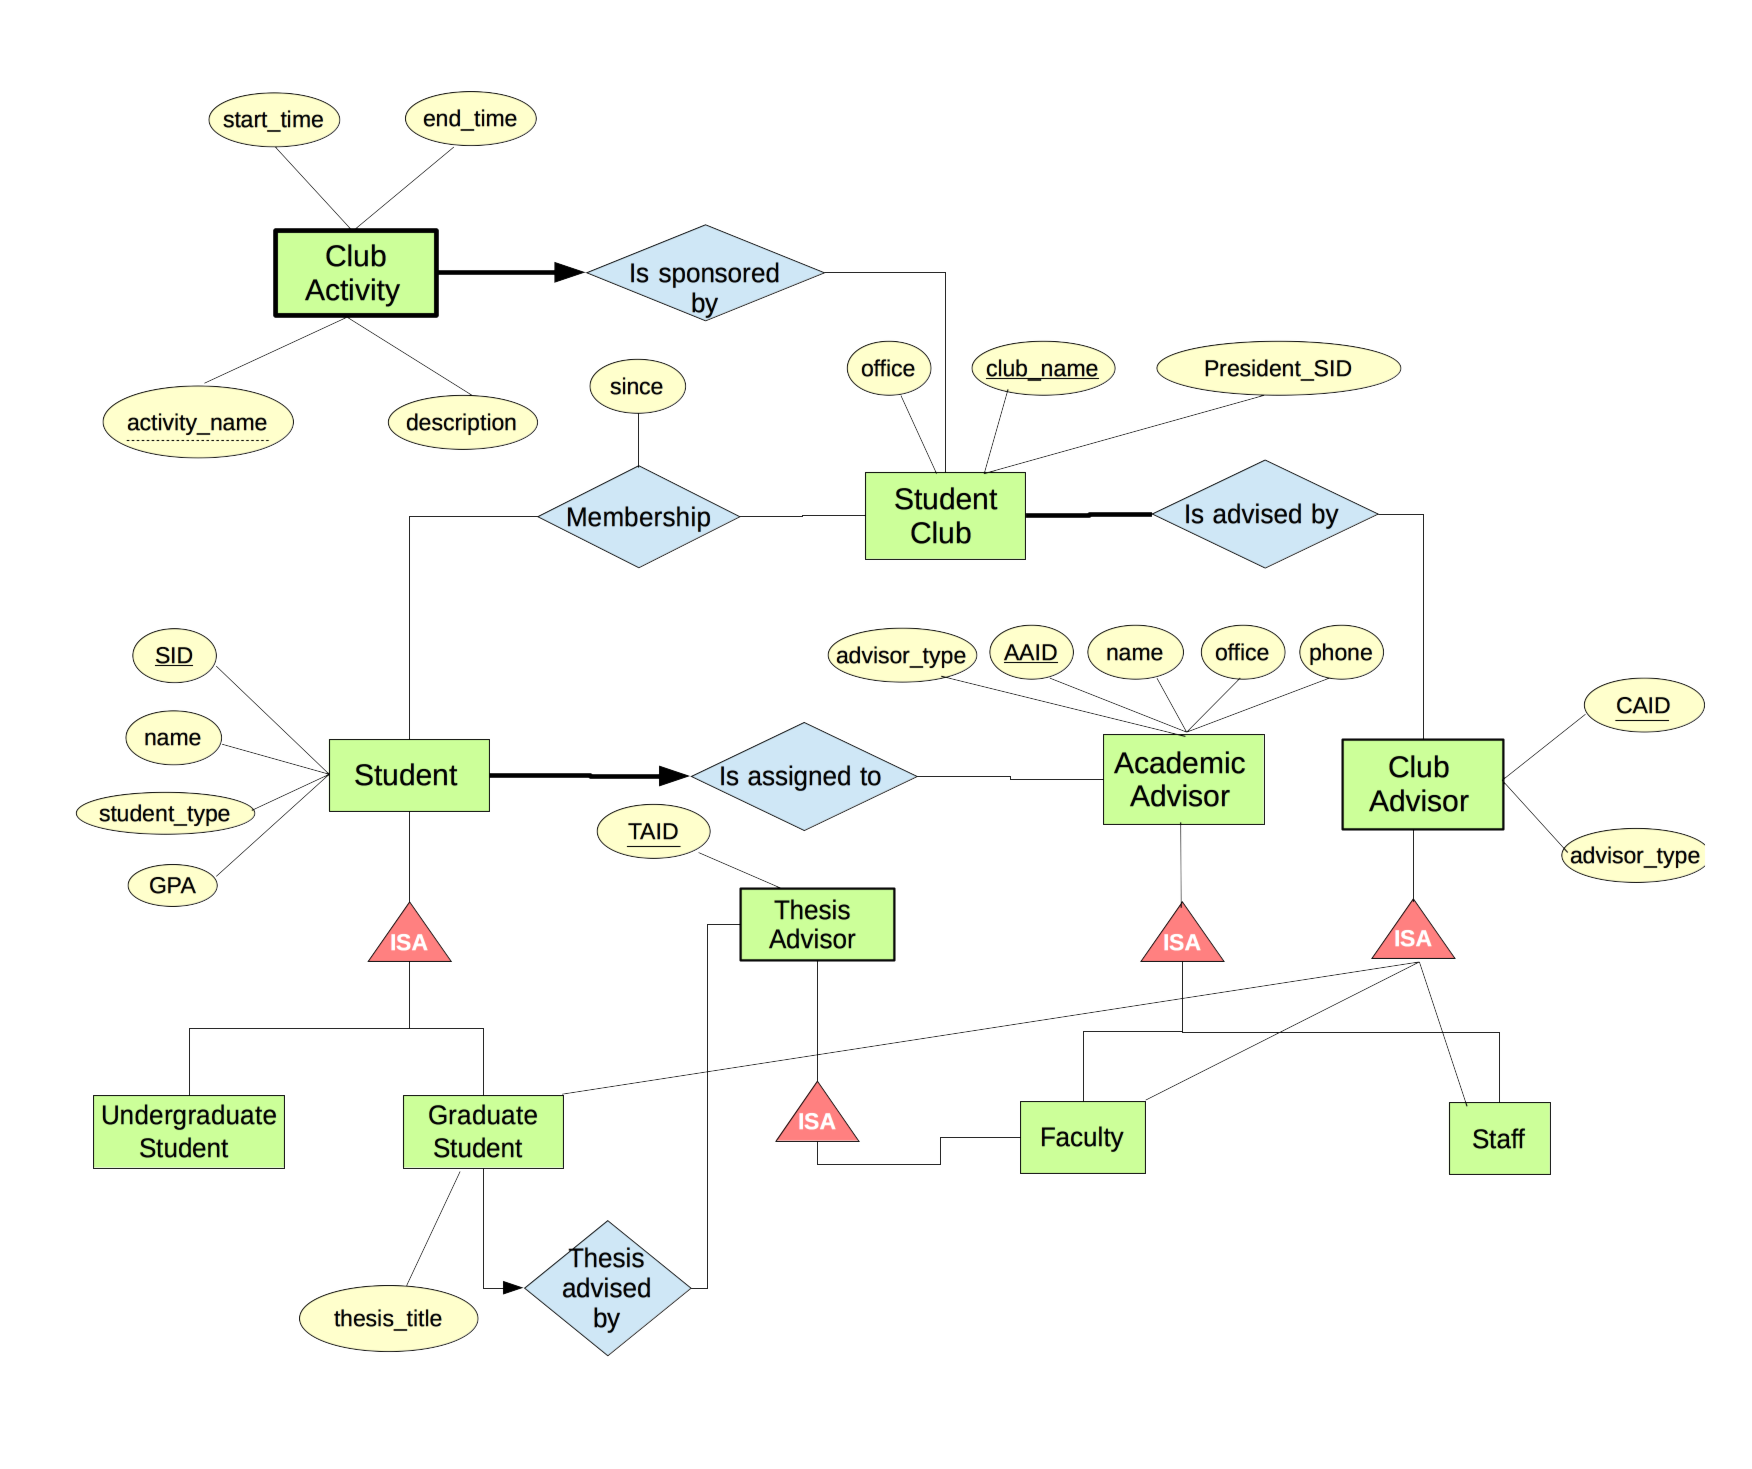
\includegraphics[width=14cm,height=12cm]{./cs460-prog4-er.png}
\end{center}

\underline{ER Symbols Explanation}:
\begin{center}
  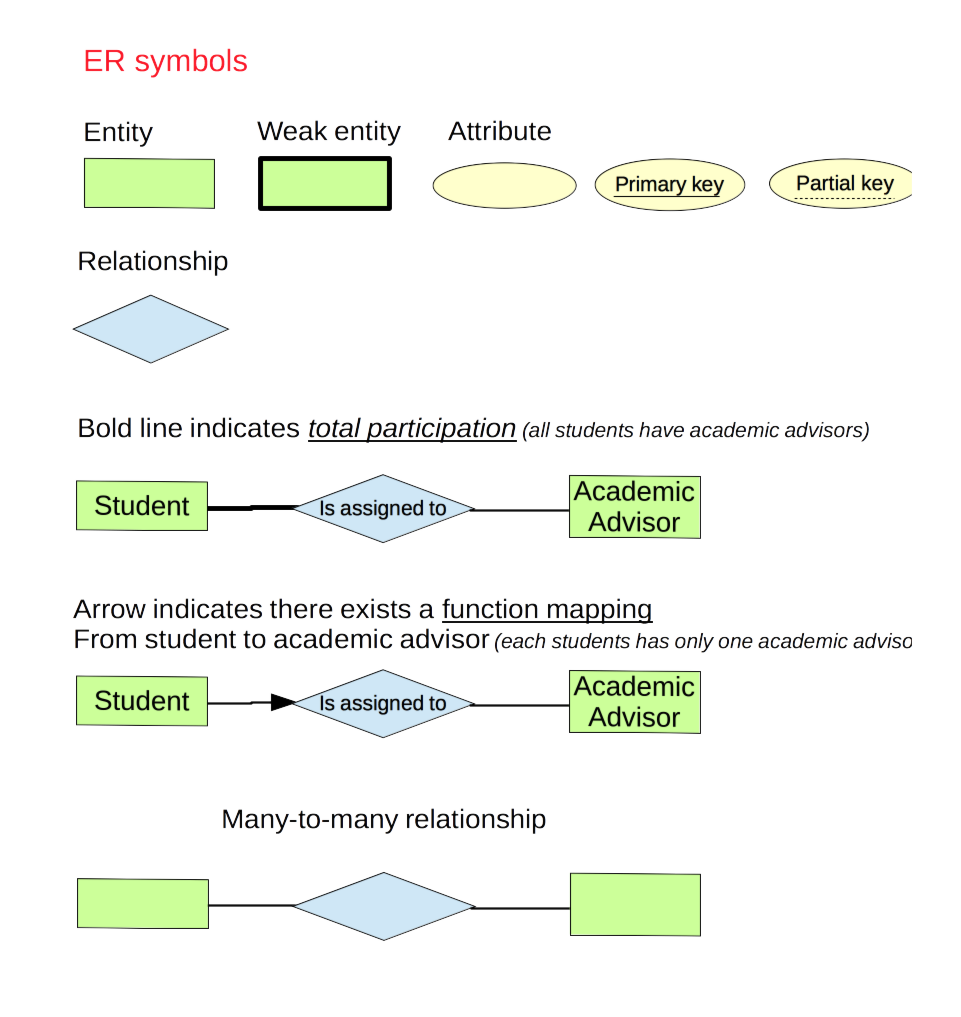
\includegraphics[width=9cm,height=10cm]{./cs460-proj4-legend.png}
\end{center}

\underline{Assumptions}:
\begin{itemize}
\item each student club can have multiple advisors; each club advisor
  can advise multiple clubs.
\item a thesis advisor can advise multiple graduate students.
\end{itemize}

\vspace{1em}
\underline{Logical Design/Relational Schema}:

\begin{enumerate}
\item \textbf{Academic\_Advisor} (\underline{AAID}, name, office,
  phone, advisor\_type)\\\\
  This table corresponds to the \texttt{Academic Advisor} entity in
  the ER diagram.\\
  \emph{\texttt{AAID} represents a unique academic advisor ID;
    \texttt{advisor\_type} can only be ``Faculty'' or ``Staff''.}

\item \textbf{Student} (\underline{SID}, name, student\_type, gpa,
  advisor\_id)\\\\
  This table corresponds to the \texttt{Student} entity in the ER
  diagram.\\
  \emph{\texttt{SID} represents a unique student ID; \texttt{advisor\_id} is the
    foreign key refers to the primary key \texttt{AAID} of the
    \texttt{Academic\_Advisor}; \texttt{student\_type} can 
    only be either ``Graduate'' or ``Undergraduate''.}

\item \textbf{Student\_Club} (\underline{club\_name}, office,
  president\_SID)\\\\
  This table corresponds to the \texttt{Student Club} entity in
  the ER diagram.\\
  \emph{\texttt{club\_name} represents a unique club name (within
    department);
    \texttt{president\_SID} is foreign key refers to the primary 
  key \texttt{SID} of the \texttt{Student} table, it's the student ID
  of the president of the club. This value cannot be
  NULL in order to satisfy the constraint that ``each
  club must have at least one member to exist''}

\item \textbf{Club\_Membership} (\underline{SID},
  \underline{club\_name}, since)\\\\
  This table corresponds to the \texttt{Membership} relationship in
  the ER diagram.\\

\item \textbf{Grad\_Club\_Advisor} (\underline{CAID},
  \underline{SID})\\\\
  This table corresponds to part of the \texttt{Club Advisor}
  entity in the ER diagram. Specifically, it represents those graduate
  students who are club advisors.\\
  \emph{\texttt{CAID} represents a unique club advisor
    ID for graduate student. \texttt{SID} is the 
    foreign key refers to the primary key \texttt{SID} of the
    \texttt{Student} table. Namely, the student ID of the graduate
    student who advises a club.}

\item \textbf{Faculty\_Staff\_Club\_Advisor} (\underline{CAID},
  \underline{AAID})\\\\
  This table corresponds to part of the \texttt{Club Advisor}
  entity in the ER diagram. Specifically, it represents those faculty
  and staff who are club advisors.\\
  \emph{\texttt{CAID} represents a unique club advisor ID for faculty
    and staff. \texttt{AAID} is the
    foreign key refers to the primary key \texttt{AAID} of the
    \texttt{Academic Advisor} table. Namely, the academic adviosr ID
    of the faculty or staff who advises a club.}

\item \textbf{Club\_Advised\_By} (\underline{CAID},
  \underline{club\_name}, \underline{advisor\_type})\\\\
  This table corresponds to the \texttt{is advised by} relationship in
  the ER diagram.\\
  \emph{\texttt{CAID} is the
    foreign key refers to the primary key \texttt{CAID} of either
    \texttt{Faculty\_Staff\_Club\_Advisor} or
    \texttt{Grad\_Club\_Advisor} table depends on the value of
    \texttt{advisor\_type}. \texttt{advisor\_type} can 
    only be either ``Faculty\_Staff'' or ``Graduate\_Student''.}

\item \textbf{Club\_Activity} (\underline{activity\_name},
  \underline{club\_name}, start\_time, end\_time)\\\\
  This table corresponds to the \texttt{Club Activity} entity in
  the ER diagram.\\

\item \textbf{Thesis\_Advised\_By} (\underline{SID}, AAID,
  thesis\_title)\\\\
  This table corresponds to the \texttt{Thesis advised by}
  relationship in the ER diagram.\\
  \emph{\texttt{SID} is the student ID of the graduate who has a
    thesis advisor. \texttt{AAID} is the academic advisor ID of the
    faculty who advises the thesis.}

\end{enumerate}

\underline{Design Decisions}:

\vspace{1em}
\begin{itemize}
\item $AAID$ and $CAID$ are treated differently. $AAID$ is
  pre-assigned to each faculty and staff member, 
  regardless they are currently advising students or not. $CAID$ are
  generated as needed, if a club advisor no longer advises a club,
  his/her $CAID$ will be deleted.
\item Because club advisor can be graduate student, faculty or staff,
  we need two relations: \textbf{Grad\_Club\_Advisor} and
  \textbf{Faculty\_Staff\_Club\_Advisor} for the entity \textbf{Club
    Advisor} in the conceptual design.
\item $CAID$ are not unique across \textbf{Grad\_Club\_Advisor} and
  \textbf{Faculty\_Staff\_Club\_Advisor} relations. It's only unique
  within each relation. So it's possible to have both a graduate
  student and a faculty member with $CAID$ of $1$.
\item Since not every graduate student has a thesis advisor, so it is
  not a good practice to store thesis advisor ID directly in
  \textbf{Student} relation, because then we will have a lot of NULL
  foreign keys.
\item All the information regarding to graduate student is captured in
  \textbf{Thesis\_Advised\_By} relation, so there is no need to have a
  specific relation for graduate student.
\item There is no need to have specific relations for undergraduate
  student, faculty or staff unless there are information specific to
  these three entities we need to model, for example, faculty may have
  research areas they are focusing on, staff may have specific duties
  to perform.
\end{itemize}


\underline{Normalization Analysis}:

\vspace{1em}
Recall that a relation $R$ is in 3NF if and only if both of the
following conditions holds:
\begin{itemize}
\item $R$ is in 2NF.
\item Every non-prime attribute of $R$ is non-transitively dependent
  on every key of $R$.
\end{itemize}

A relation $R$ is in 2NF if it is in 1NF and every non-prime attribute
of the table is dependent on the whole of every candidate key. (no
partial dependency)\\

A relation $R$ is in 1NF if the value of each attribute contains only
a single value from its corresponding domain which contains only
atomic values.

Note that trivial FDs are ignored in the following analysis.

\begin{enumerate}
\item \textbf{Academic\_Advisor} (\underline{AAID}, name, office,
  phone, advisor\_type)

  Candidate key: $AAID$\\
  Primary key: $AAID$

  FDs: $AAID \rightarrow name$; $AAID \rightarrow office$; $AAID
  \rightarrow phone$; $AAID \rightarrow advisor\_type$;

  The table is in 1NF assuming that each advisor can only have a
  single office and a phone.

  The table is in 2NF because the only candidate key contains a single
  attribute, there is no partial dependency in this table.

  The table is in 3NF because the only candidate key contains a single
  attribute and there are no FDs existing among non-prime attributes.

\item \textbf{Student} (\underline{SID}, name, student\_type, gpa,
  advisor\_id)

  Candidate key: $SID$\\
  Primary key: $SID$

  FDs: $SID \rightarrow name$; $SID \rightarrow gpa$; $SID
  \rightarrow advisor\_id$; $SID \rightarrow student\_type$;

  The table is in 1NF assuming that each student has only one name,
  advisor, gpa and is either graduate or undergraduate student.

  The table is in 2NF because the only candidate key contains a single
  attribute, there is no partial dependency in this table.

  The table is in 3NF because the only candidate key contains a single
  attribute and there are no FDs existing among non-prime attributes.

\item \textbf{Student\_Club} (\underline{club\_name}, office,
  president\_SID)

  Candidate key: $club\_name$\\
  Primary key: $club\_name$

  FDs: $club\_name \rightarrow office$; $club\_name \rightarrow
  president\_SID$;

  The table is in 1NF assuming that each student club has only one
  office and one president who is a student.

  The table is in 2NF because the only candidate key contains a single
  attribute, there is no partial dependency in this table.

  The table is in 3NF because the only candidate key contains a single
  attribute and there are no FDs existing among non-prime attributes.

\item \textbf{Club\_Membership} (\underline{SID},
  \underline{club\_name}, since)

  Candidate key: $\{SID, club\_name\}$\\
  Primary key: $\{SID, club\_name\}$

  FDs: $\{SID, club\_name\} \rightarrow since$;

  The table is in 1NF because each student joined a club at a specific
  time.

  The table is in 2NF because neither $SID$ nor $club\_name$ can
  functionally determine $since$.

  The table is in 3NF because there only a single non-prime
  attribute $since$ in this relation and it doesn't functionally
  determine $SID$ or $club\_name$, that means there is no transitive
  dependency in this relation.

\item \textbf{Grad\_Club\_Advisor} (\underline{CAID},
  \underline{SID})
  
  Candidate key: $CAID$, $SID$\\
  Primary key: $CAID$

  FDs: $CASID \rightarrow SID$; $SID \rightarrow CAID$;

  The table is in 1NF assuming that each graduate student has been
  assigned with only one $CAID$.

  The table is in 2NF and 3NF because there are no non-prime
  attributes in the relation.

\item \textbf{Faculty\_Staff\_Club\_Advisor} (\underline{CAID},
  \underline{AAID})

  Candidate key: $CAID$, $AAID$\\
  Primary key: $CAID$

  FDs: $CASID \rightarrow AAID$; $AAID \rightarrow CAID$;

  The table is in 1NF assuming that each faculty or staff has been
  assigned with only one $CAID$.

  The table is in 2NF and 3NF because there are no non-prime
  attributes in the relation.

\item \textbf{Club\_Advised\_By} (\underline{CAID},
  \underline{club\_name}, \underline{advisor\_type})

  Candidate key: $\{CAID, club\_name, advisor\_type\}$\\
  Primary key: $\{CAID, club\_name, advisor\_type\}$

  FDs: 

  The table is in 1NF, 2NF and 3NF because there are no non-prime
  attributes in the relation.

  Note that $CAID$ doesn't functionally determine $club\_name$ because
  a graduate student with $CAID=1$ could advise club ``A'', while a
  faculty with $CAID=1$ could advise club ``B''. Vice versa.

\item \textbf{Club\_Activity} (\underline{activity\_name},
  \underline{club\_name}, start\_time, end\_time)

  Candidate key: $\{club\_name, activity\_name\}$\\
  Primary key: $\{club\_name, activity\_name\}$

  FDs: $\{club\_name, activity\_name\} \rightarrow start\_time$;
  $\{club\_name, activity\_name\} \rightarrow end\_time$

  The table is in 1NF because each activity starts and ends at a
  specific time.

  The table is in 2NF because neither $activity\_name$ nor
  $club\_name$ can functionally determine $start\_time$ or
  $end\_time$.

  The table is in 3NF because there are no FDs existing among
  non-prime attributes and no non-prime attributes can functionally
  determine prime attributes.

\item \textbf{Thesis\_Advised\_By} (\underline{SID}, AAID,
  thesis\_title)

  Candidate key: $SID$\\
  Primary key: $SID$

  FDs: $SID \rightarrow AAID$; $SID \rightarrow thesis\_title$;

  The table is in 1NF assuming that each student has been assigned
  with only one thesis advisor and work on one thesis topic.

  The table is in 2NF because the only candidate key contains a single
  attribute, there is no partial dependency in this table.

  The table is in 3NF because the only candidate key contains a single
  attribute and there are no FDs existing among non-prime attributes.

\end{enumerate}

\vspace{1em}

\end{document}
